\documentclass[10pt,a4paper]{article}

\usepackage[margin=1.05in]{geometry}
\usepackage{setspace,amsmath,amssymb,amsthm}
\usepackage{graphicx,enumitem,titlesec,fancyhdr,microtype,hyperref}
\graphicspath{{drawings/}}

\hypersetup{colorlinks=true,linkcolor=black,urlcolor=black,citecolor=black}
\titleformat{\section}{\normalsize\bfseries}{}{0em}{}
\titleformat{\subsection}{\small\bfseries}{}{0em}{}
\titlespacing*{\section}{0pt}{1.35em}{0.5em}

\theoremstyle{plain}
\newtheorem{proposition}{Proposition}
\newtheorem{lemma}{Lemma}
\newtheorem{theorem}{Theorem}
\theoremstyle{definition}
\newtheorem{definition}{Definition}
\theoremstyle{remark}
\newtheorem{observation}{Observation}

\setstretch{1.14}
\pagestyle{fancy}
\fancyhf{}
\fancyhead[L]{\small\itshape Elements of Position}
\fancyhead[R]{\small\itshape Exploratory.\ The Cut}
\fancyfoot[C]{\small\thepage}
\renewcommand{\headrulewidth}{0pt}

\begin{document}

\begin{center}
\vspace*{1.6em}
{\large Elements of Position}\\[0.6em]
{\small Exploratory reading}\\[1.2em]
{\LARGE\bfseries The Cut}\\[0.5em]
{\small Every meeting that can be seated sits on the line the unit already had}\\[1.6em]
{\normalsize Justin Erholtz}\\[0.25em]
{\small 24 September 2026}
\end{center}

\vspace{1.0em}

\begin{center}
{\large Where is \(1\)? On the cut.}
\end{center}

\vspace{0.9em}

\noindent
The frozen parts built the object without this question.
I named the pair and the lock.
II walked: shear then bind; a hit is a sign change; two mixes that must not be crushed.
III wrote the residual as an object.
IV sat two streets on the \(1/2\) line and married them at five.
V asked what else was already true of the leftover and the tree.

This paper takes that object and reads plan, section, and elevation of the same finished stations together.
The stock of that reading is written by
\texttt{exploratory/rh/kernel.py}
into
\texttt{runs/2026-09-24\_n200/}.
A later classical name may be used for the reading.
It does not get the first word.
The cut does.

\vspace{0.7em}
\noindent
\textit{A note.}
Identities of the pair are citations of I.
The walk run remains
\texttt{kernels/walk/runs/2026-09-24\_h0.002\_n200000/}.
Those two clocks are not one list.
A claim that can be proved by school geometry is proved that way.
A claim that names a classical limit is named as an identification, after the drawings exist together.
The \(t\)-grid of the first kernel run is five heights.
It is not a search for ordinates.

\tableofcontents

\section{What is already on the page}

The unit closes; the interior does not.
The pair is \((n,1/n)\), product \(1\), geometric mean \(1\).
The leftover \(\tau(n)=(n-1)^2/(2n)\) vanishes only at the lock \(n=1\).

The heading moves by \(T_h\) then bind.
No angle is an argument of either move.
A hit is a sign change of the second coordinate.
On the recorded kick: \(h=0.002\), \(H_0=1571\), \(127\) hits, two gap integers.

Two mixes stay split.
\(h=\tan(\pi/n)\) writes one gap letter \(n\).
\(h=\tan(2\pi/n)\) writes the n-gon vertex.
At five those are not the same kick.
Marriage is the vertex mix together with \(2\cos(\pi/5)=\varphi\), checked on the 24~September n-gon and bridge tables.

The even cut of every finished segment is \(1/2\).
IV already sat both streets on that line.

The master count \(n=1,2,\ldots\) is the ruler of I.
At each \(n\) the kernel writes origin \(n/2\) and inverse \(1/n\).
On the first run, \(n\le 200\), forty-six of those stations are irreducible.
\(n=1\): origin \(1/2\), inverse \(1\). The lock.
\(n=2\): origin \(1\), inverse \(1/2\).
\(n=5\): origin \(5/2\), inverse \(1/5\).
Hit index \(m\) from the walk is a different clock.

\begin{figure}[htbp]
\centering
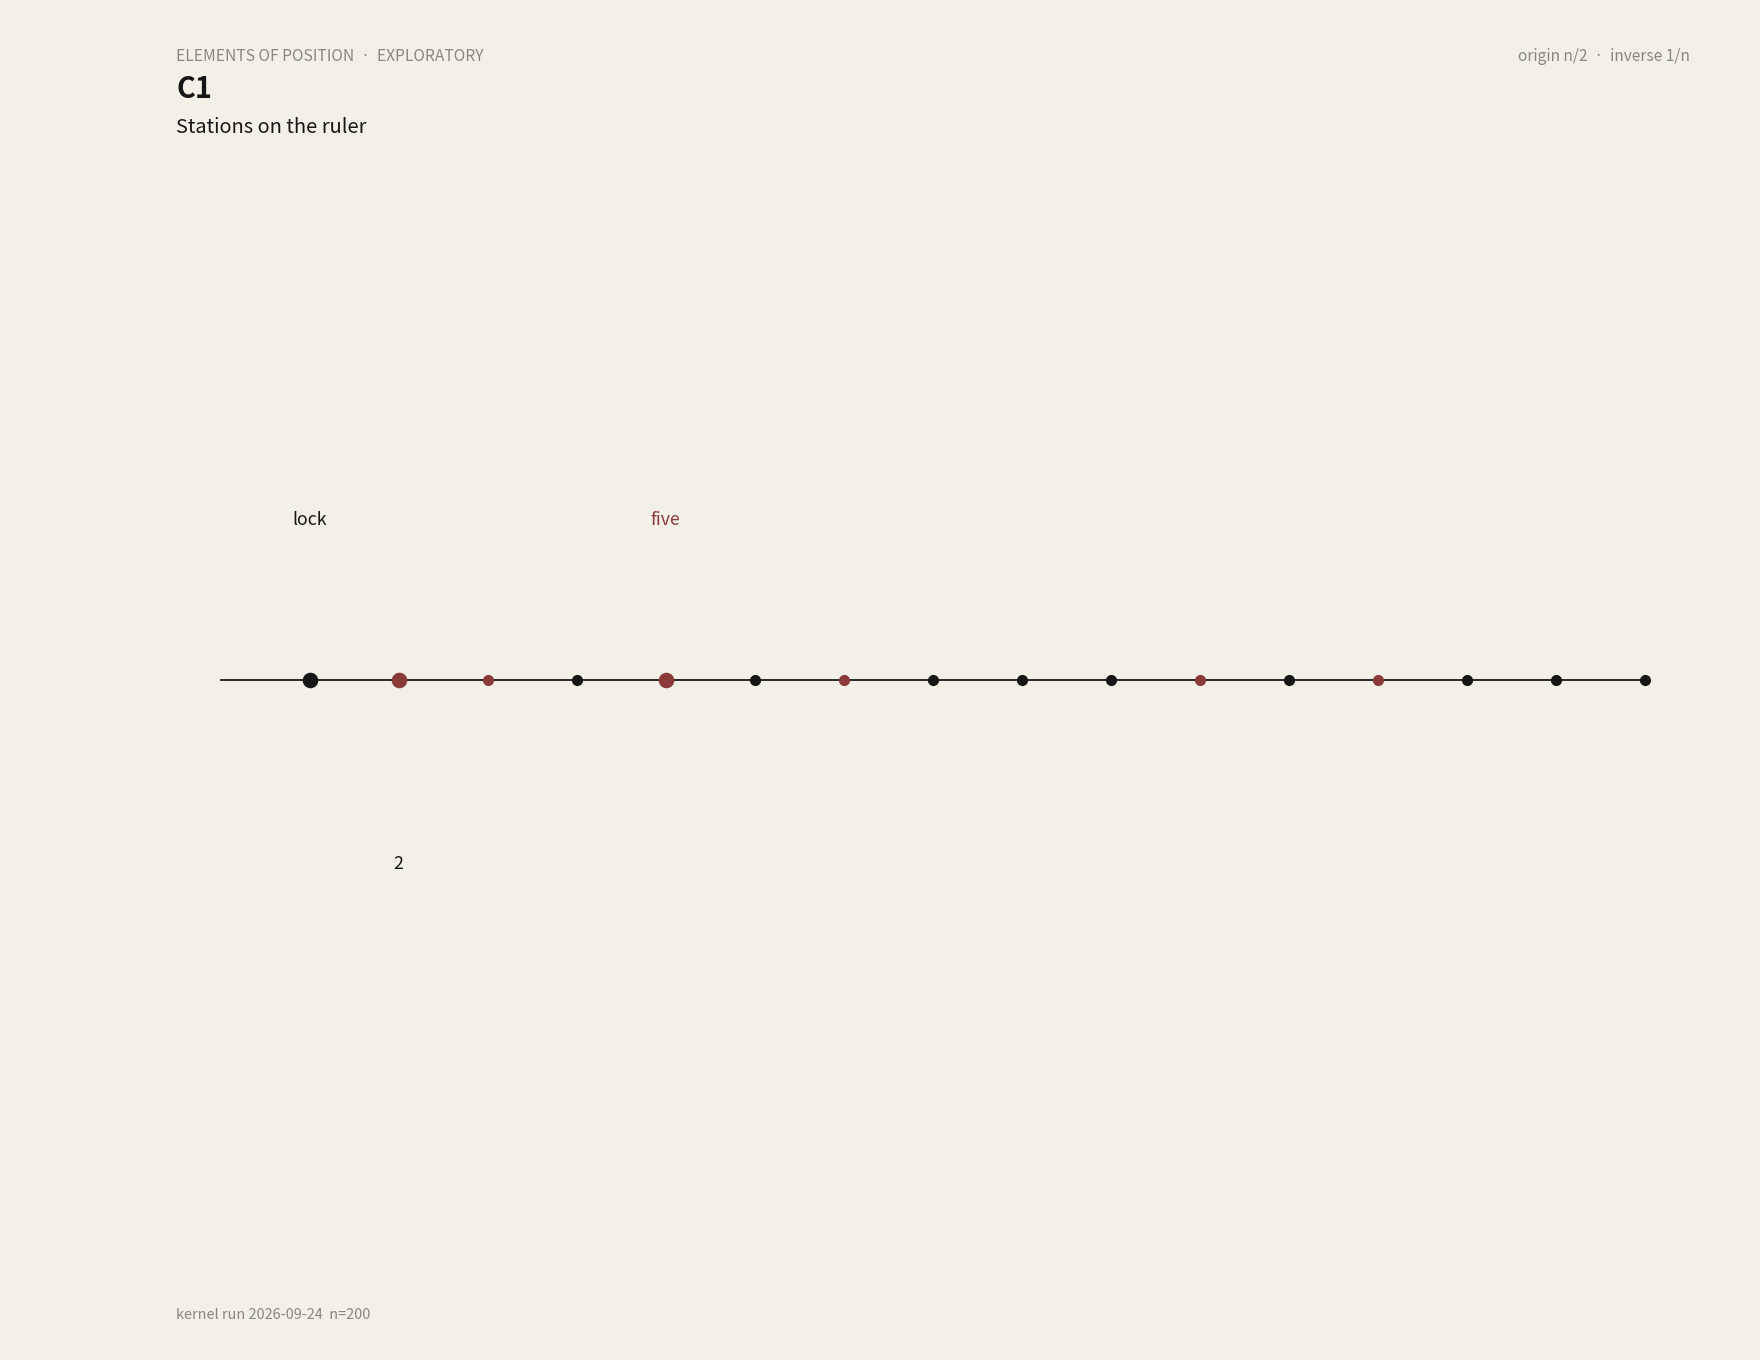
\includegraphics[width=0.92\textwidth]{C1_stations.png}
\caption{Sheet C1. First sixteen stations. Accent marks irreducibles.}
\end{figure}

\section{Vacuum, trace, pause}

Vacuum is the respect in which a relation may be named without being walked.
\(x\mapsto 1/x\) can be written in one stroke.

Trace is the same relation inscribed as positions.
II is that inscription.

Rate \(0\) is pause: process off, no next tick.
What remains live is the local circle already owned at that station --- the n-gon convention, diameter \(n\), radius \(n/2\).
Rate other than \(0\) is the count moving.
Stopping does not mint a second centre.

Naming is not arrival.
Treat a name as a seat and privilege returns by the back door.

\section{Complementary interiors}

Look-back from a pause is logarithm; live ticks are additive.
The invariant of inversion is \(dx/x\); along a finished arrival \(n>1\) that integral is \(\log n\).

Let \(\alpha\) be signed distance from \(1/2\), and set \(\sigma=\tfrac12+\alpha\).
The inversion pair with \(x=n^{\alpha}\) is \(\{n^{\alpha},n^{-\alpha}\}\).
Multiply through by \(n^{-1/2}\):
\[
\{n^{-\sigma},\,n^{-(1-\sigma)}\}.
\]

\begin{lemma}[Weights]
At a finished arrival \(n>1\), the pair \(\{n^{-\sigma},\,n^{-(1-\sigma)}\}\) has geometric mean \(n^{-1/2}\) for every real \(\sigma\).
The two ends are equal if and only if \(\sigma=1/2\).
\end{lemma}

\begin{proof}
The product of the ends is \(n^{-1}\).
Equality of ends is \(\sigma=1/2\).
This is I, applied to complementary interiors.
\end{proof}

On \texttt{weights.csv} the geometric mean equals \(n^{-1/2}\) to machine precision.
The product of the ends equals \(n^{-1}\).
\(\sigma\leftrightarrow 1-\sigma\) swaps the ends.

\begin{figure}[htbp]
\centering
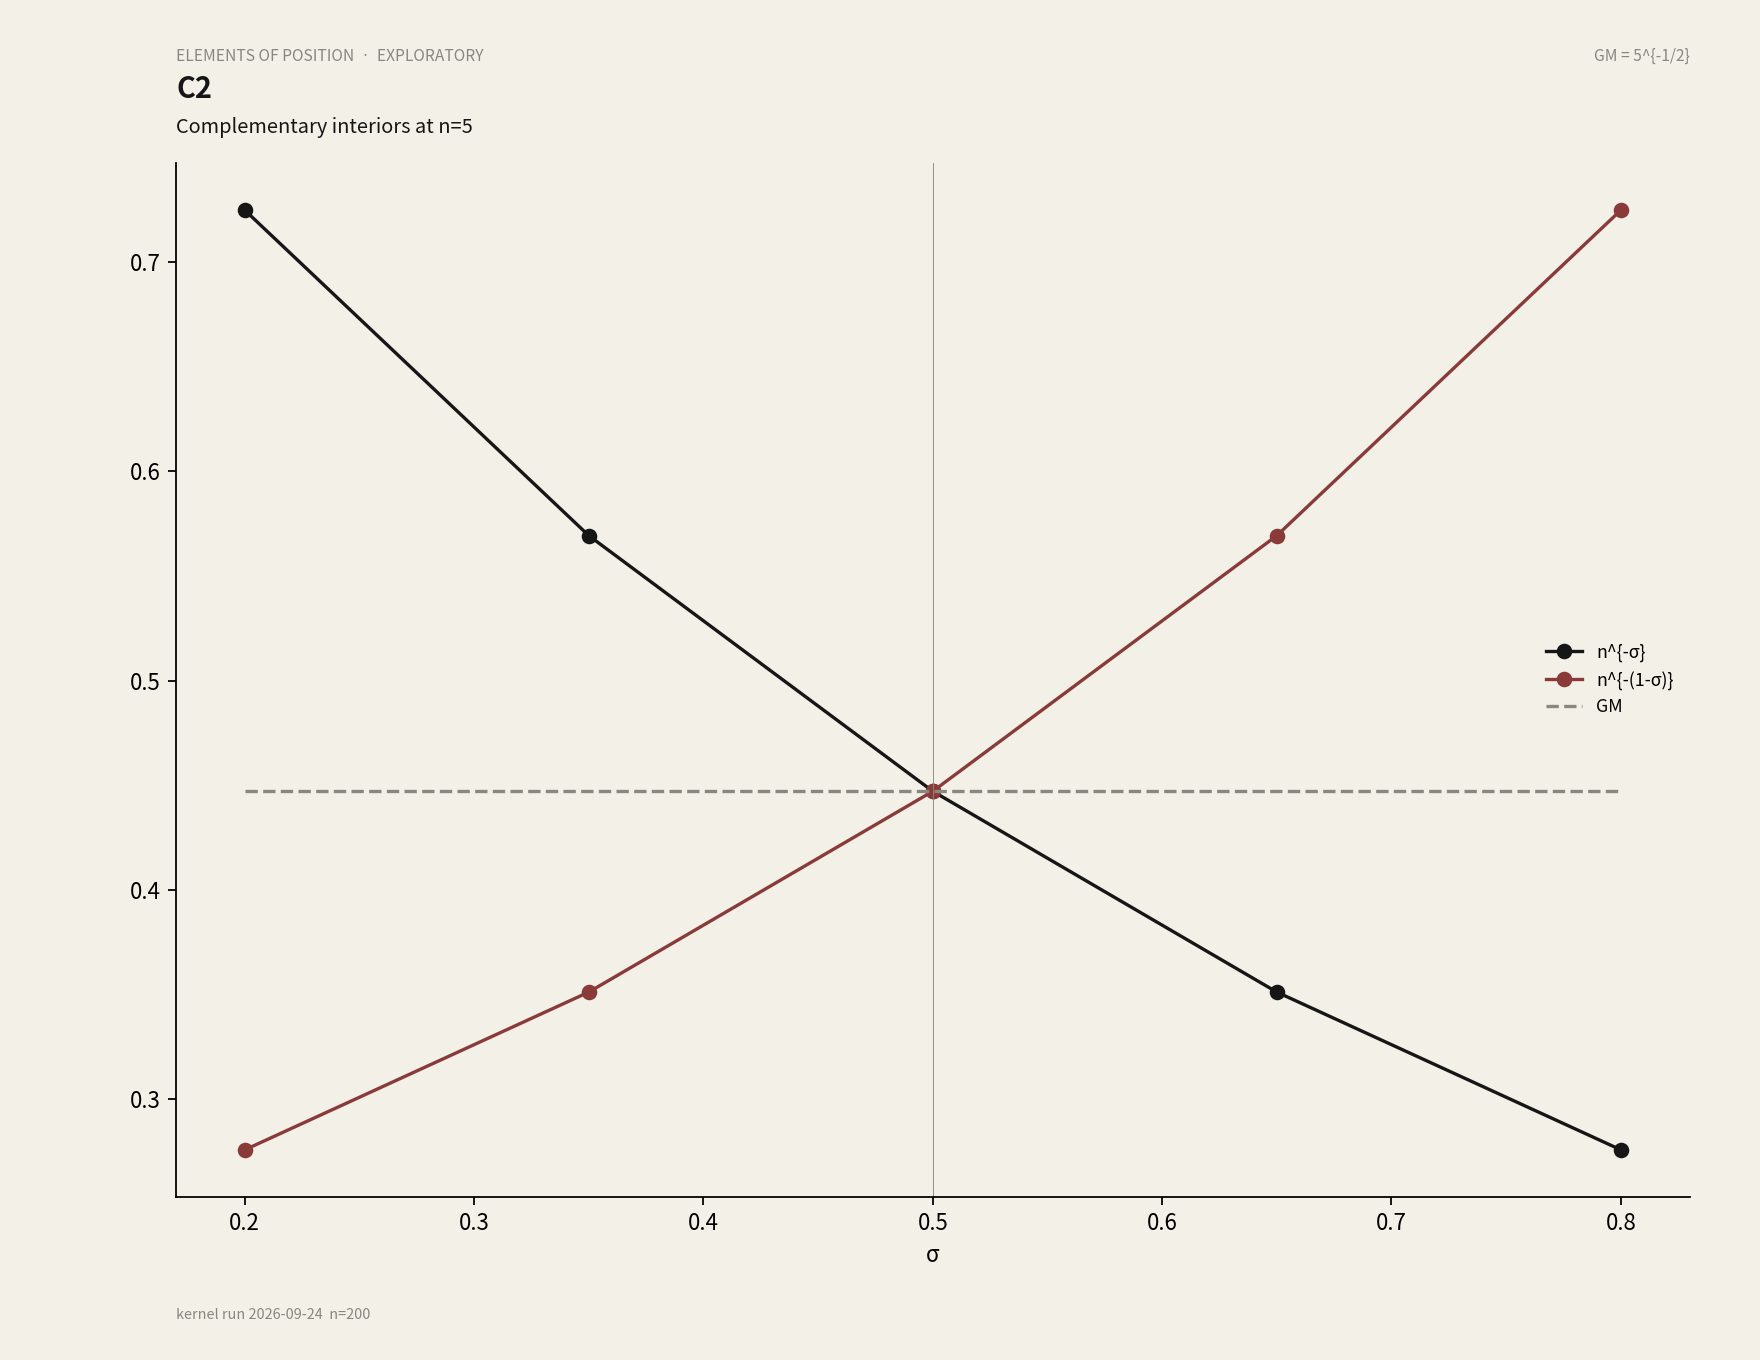
\includegraphics[width=0.92\textwidth]{C2_weights.png}
\caption{Sheet C2. Ends at $n=5$. They meet only on the cut.}
\end{figure}

\section{The only primary ratio}

\begin{lemma}[Only primary self-ratio]
On any real segment there is a unique primary, scale-invariant, \(\pm\)-equal self-description of location: the midpoint ratio \(1/2\).
\end{lemma}

The similar cuts \(\varphi\) and \(1/\varphi\) are maximal similar copies.
They sit on the same midline (IV).
They are not a second primary self-description of location.

\begin{definition}[Permanent analytic cut]
A permanent analytic cut of the derived unit is a vertical line \(\operatorname{Re}s=\sigma_0\) that functions as a primary, scale-invariant, \(\pm\)-equal self-description of location for that unit under the identification of live scale and vacuum writing.
\end{definition}

\begin{lemma}[Only permanent analytic cut]
Under that identification the only permanent analytic cut is \(\operatorname{Re}s=1/2\).
\end{lemma}

\begin{proof}
The segment \([0,1]\) in the live geometry is the strip \(0<\operatorname{Re}s<1\) in the vacuum writing of the same unit.
That pull-back is named here and not in I--V.
The midpoint of \([0,1]\) is \(1/2\).
Its image is the line \(\operatorname{Re}s=1/2\).
Any other vertical line would have to function as a second primary self-description of location for that strip.
There is no such description.
\end{proof}

Uniqueness of the cut is not yet uniqueness of every vanishing.
A pair of names \(\{\rho,1-\rho\}\) still has midpoint \(1/2\).
The pairing does not collapse the pair.
A meeting is extra: the two ends meet.

\section{What the stock can set to zero}

A finished irreducible arrival \(p\) is a station.
The data permitted there are the arrivals \(q\le p\), the local circle of radius \(p/2\), and look-back against what has already arrived.

On that station the dated product
\[
P_p(s)=\prod_{q\le p}(1-q^{-s})^{-1}
\]
is a finite object.
Each factor is never zero wherever it is defined, so the dated product never vanishes.
On \texttt{dated\_product.csv} every recorded modulus is positive.
At height \(0\), \(\sigma=0.2\), the modulus grows from \(1.4\times 10^{2}\) at \(p=5\) to \(7.0\times 10^{12}\) at \(p=199\).
At height \(14\), \(\sigma=0.2\), \(p=199\), the modulus is \(9.1\times 10^{-3}\).
Small is not a seat.

\begin{figure}[htbp]
\centering
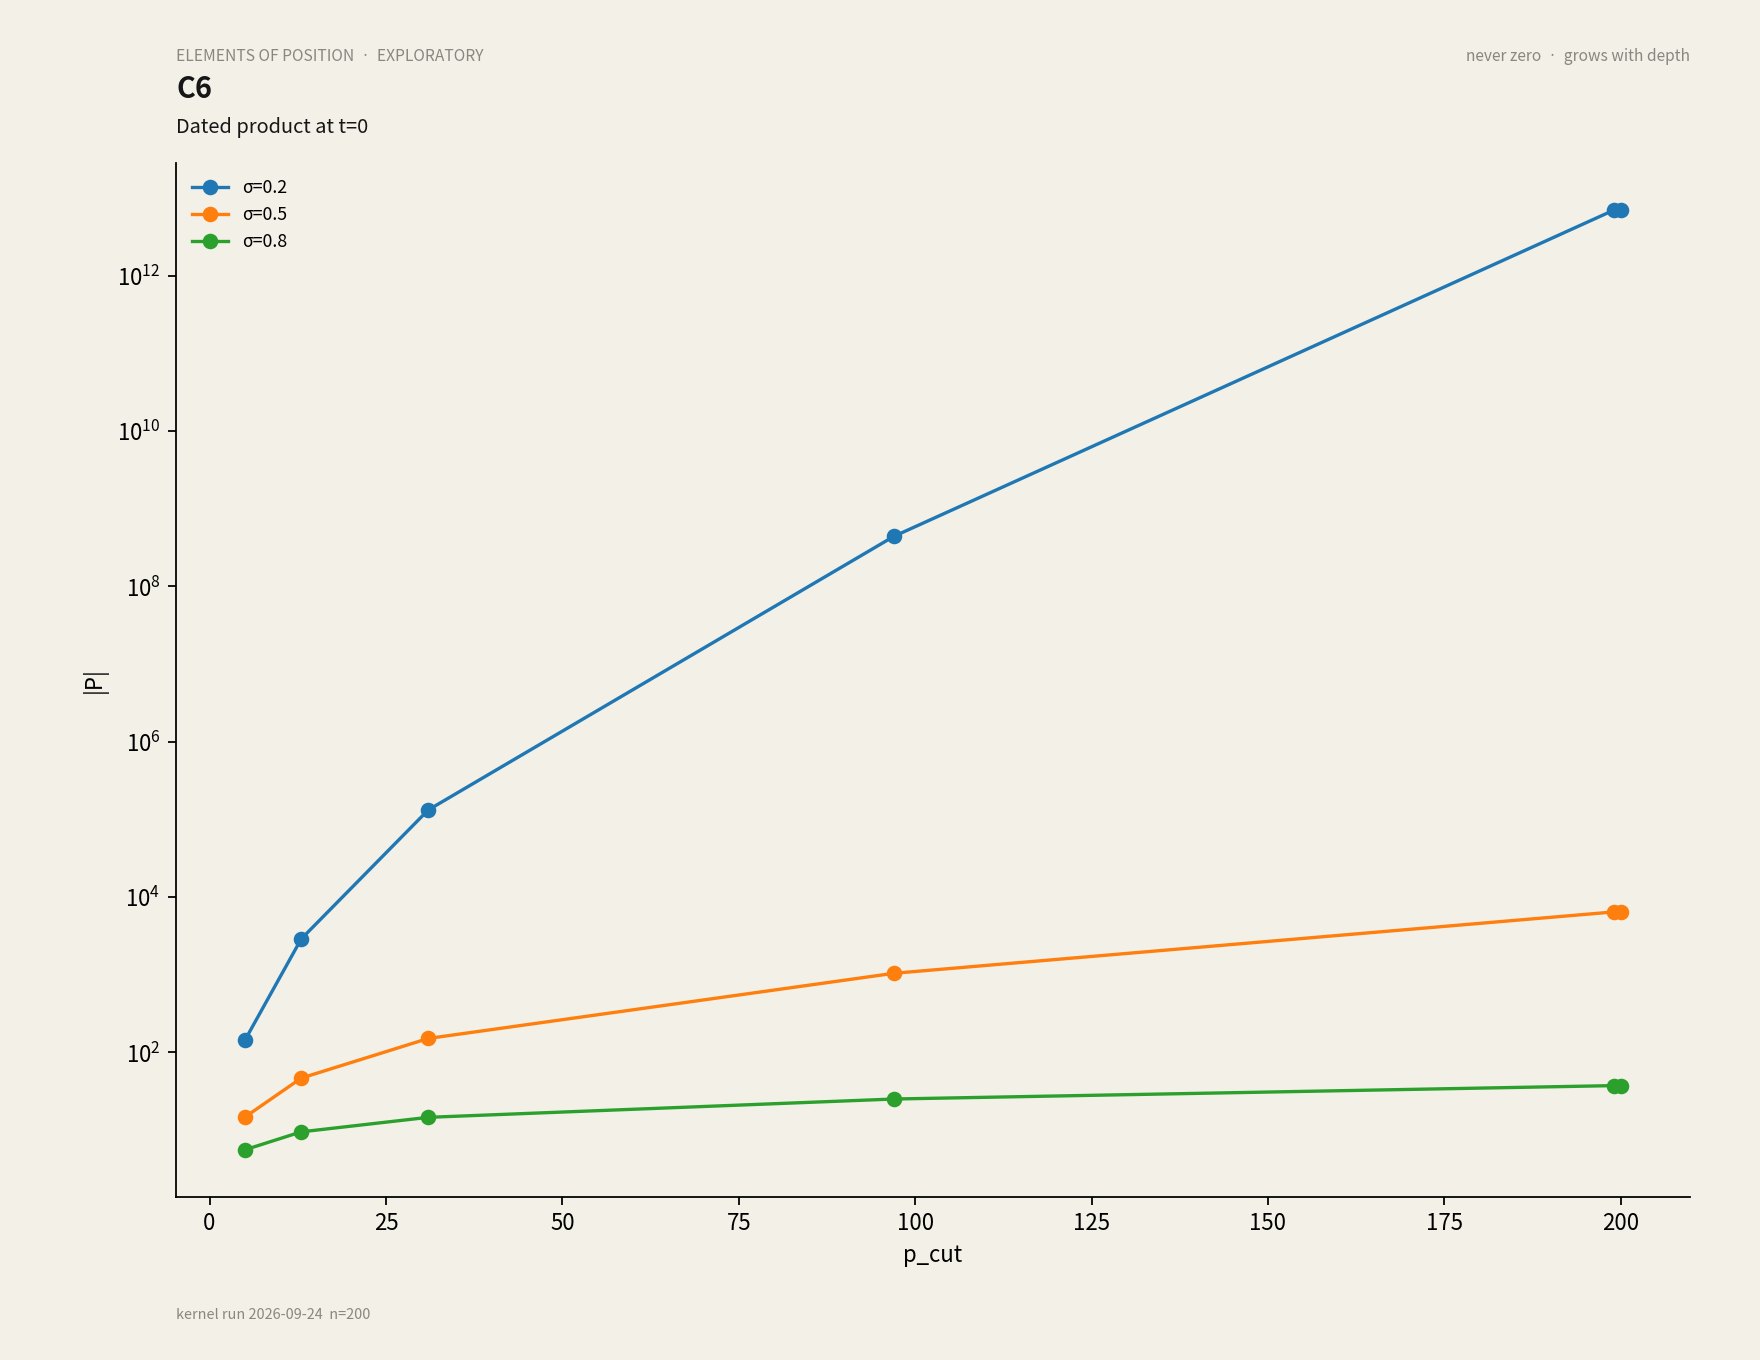
\includegraphics[width=0.92\textwidth]{C6_dated_product.png}
\caption{Sheet C6. $|P_p|$ at height $0$. No row is zero.}
\end{figure}

The local-circle sample has no zeros in \(0<\operatorname{Re}s<1\).
A midline polynomial \(\tfrac12 s(s-1)\) accounts for the endpoints \(0\) and \(1\), and stops there.

Therefore a non-trivial vanishing is not a finite-depth fact.
It appears only when stations deepen, and only in a formula that is allowed to be zero.
In this stock that formula is the dual sum of the complementary pair from the weights lemma.

\begin{theorem}[Only vanishing mechanism]
In the strip \(0<\operatorname{Re}s<1\), the only formula in the stock that can vanish non-trivially is the dual sum of the pair.
\end{theorem}

The product cannot do it.
The circle cannot do it.
The sum of the two ends is what remains.

At height \(0\) and \(N=200\),
\[
S(1/2)=51.71851469268677=\sum_{n=2}^{200}2n^{-1/2},
\]
and \(S(0.2)=S(0.8)=94.079\).
The recorded floor is the cut.
\texttt{dual\_height.csv} keeps \(\lvert S(\sigma,t)\rvert=\lvert S(1-\sigma,t)\rvert\).
On the cut the sum is real.
The first run does not list a root.

\begin{figure}[htbp]
\centering
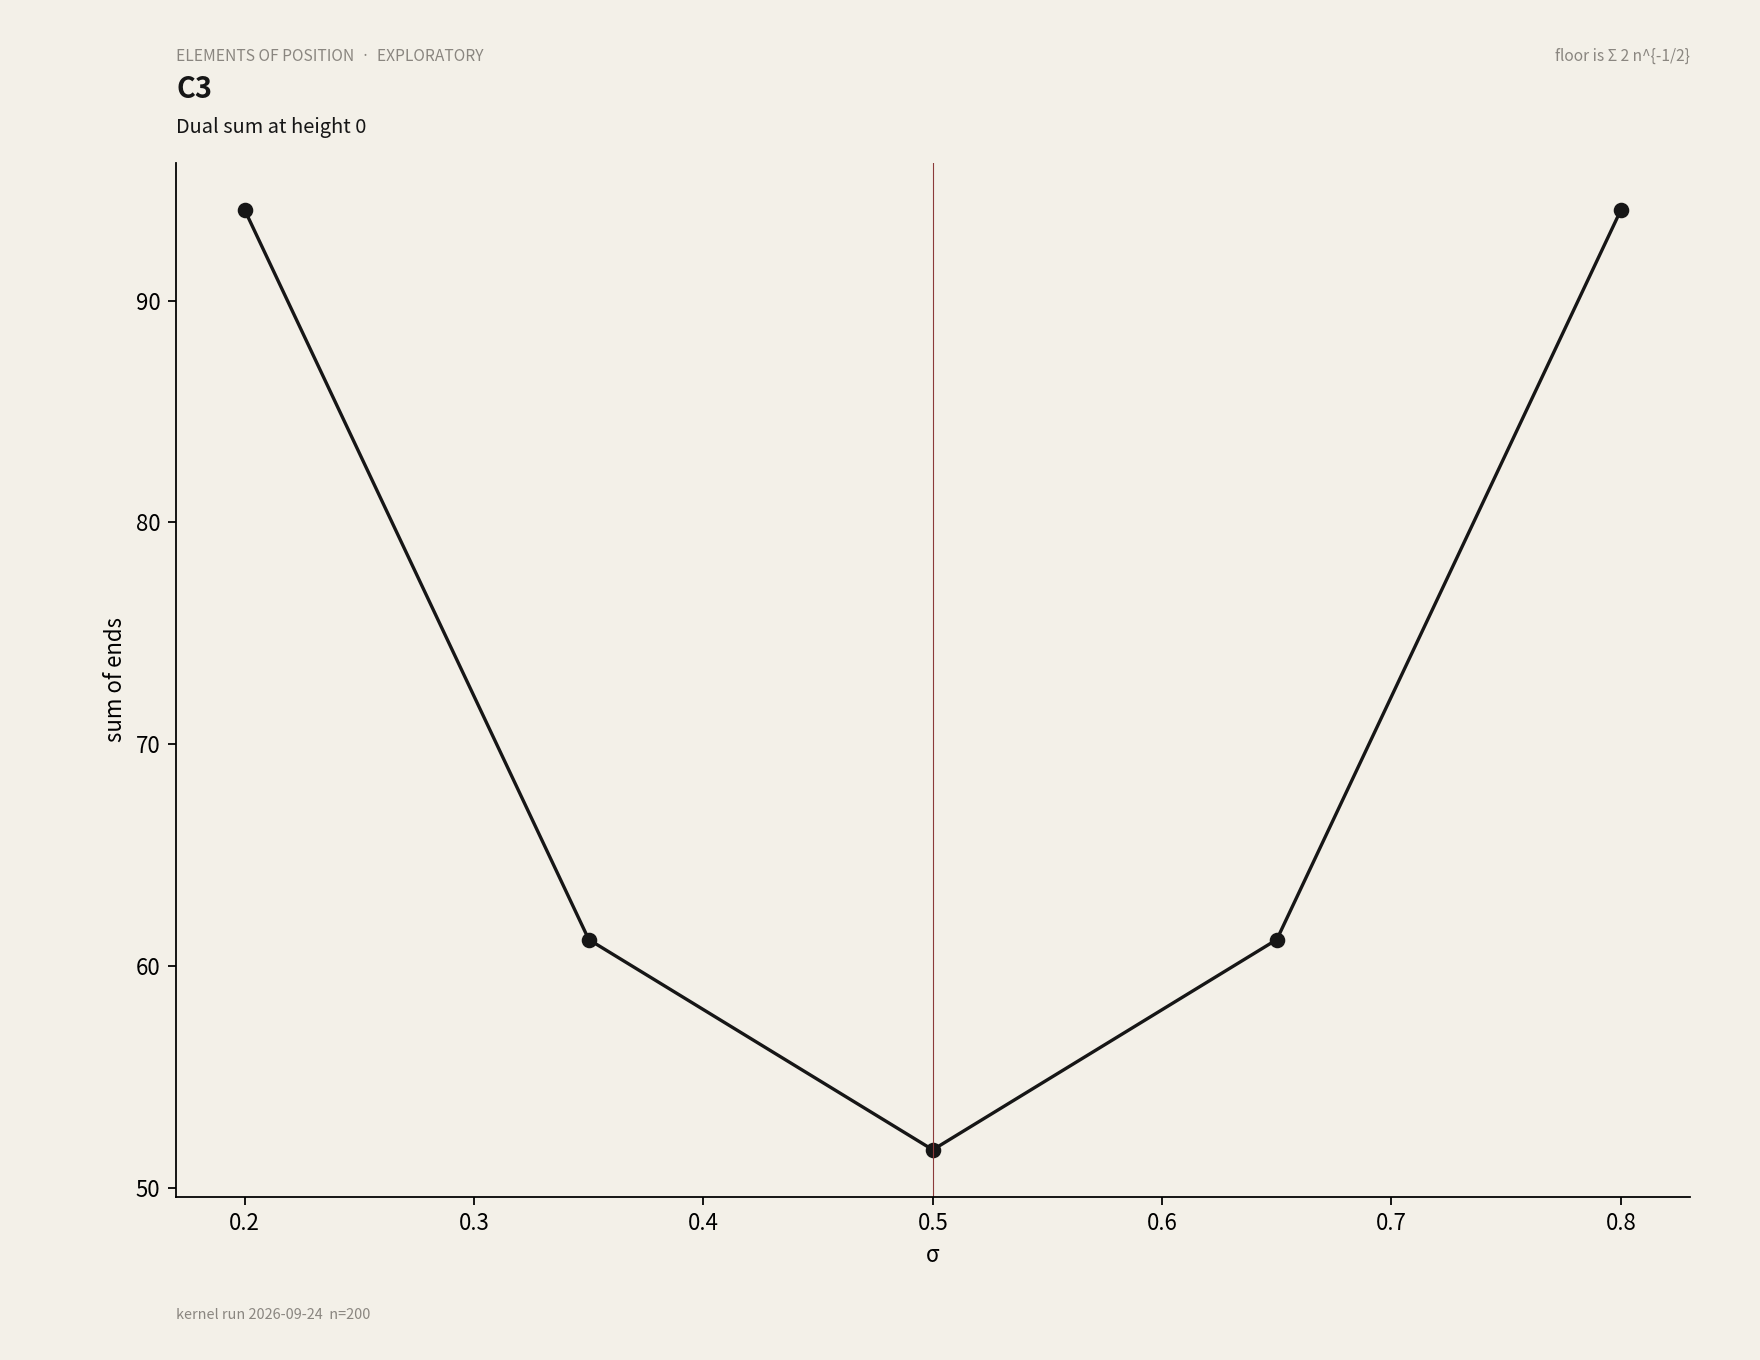
\includegraphics[width=0.92\textwidth]{C3_dual_real.png}
\caption{Sheet C3. Dual sum at height $0$. The floor is the cut.}
\end{figure}

\begin{figure}[htbp]
\centering
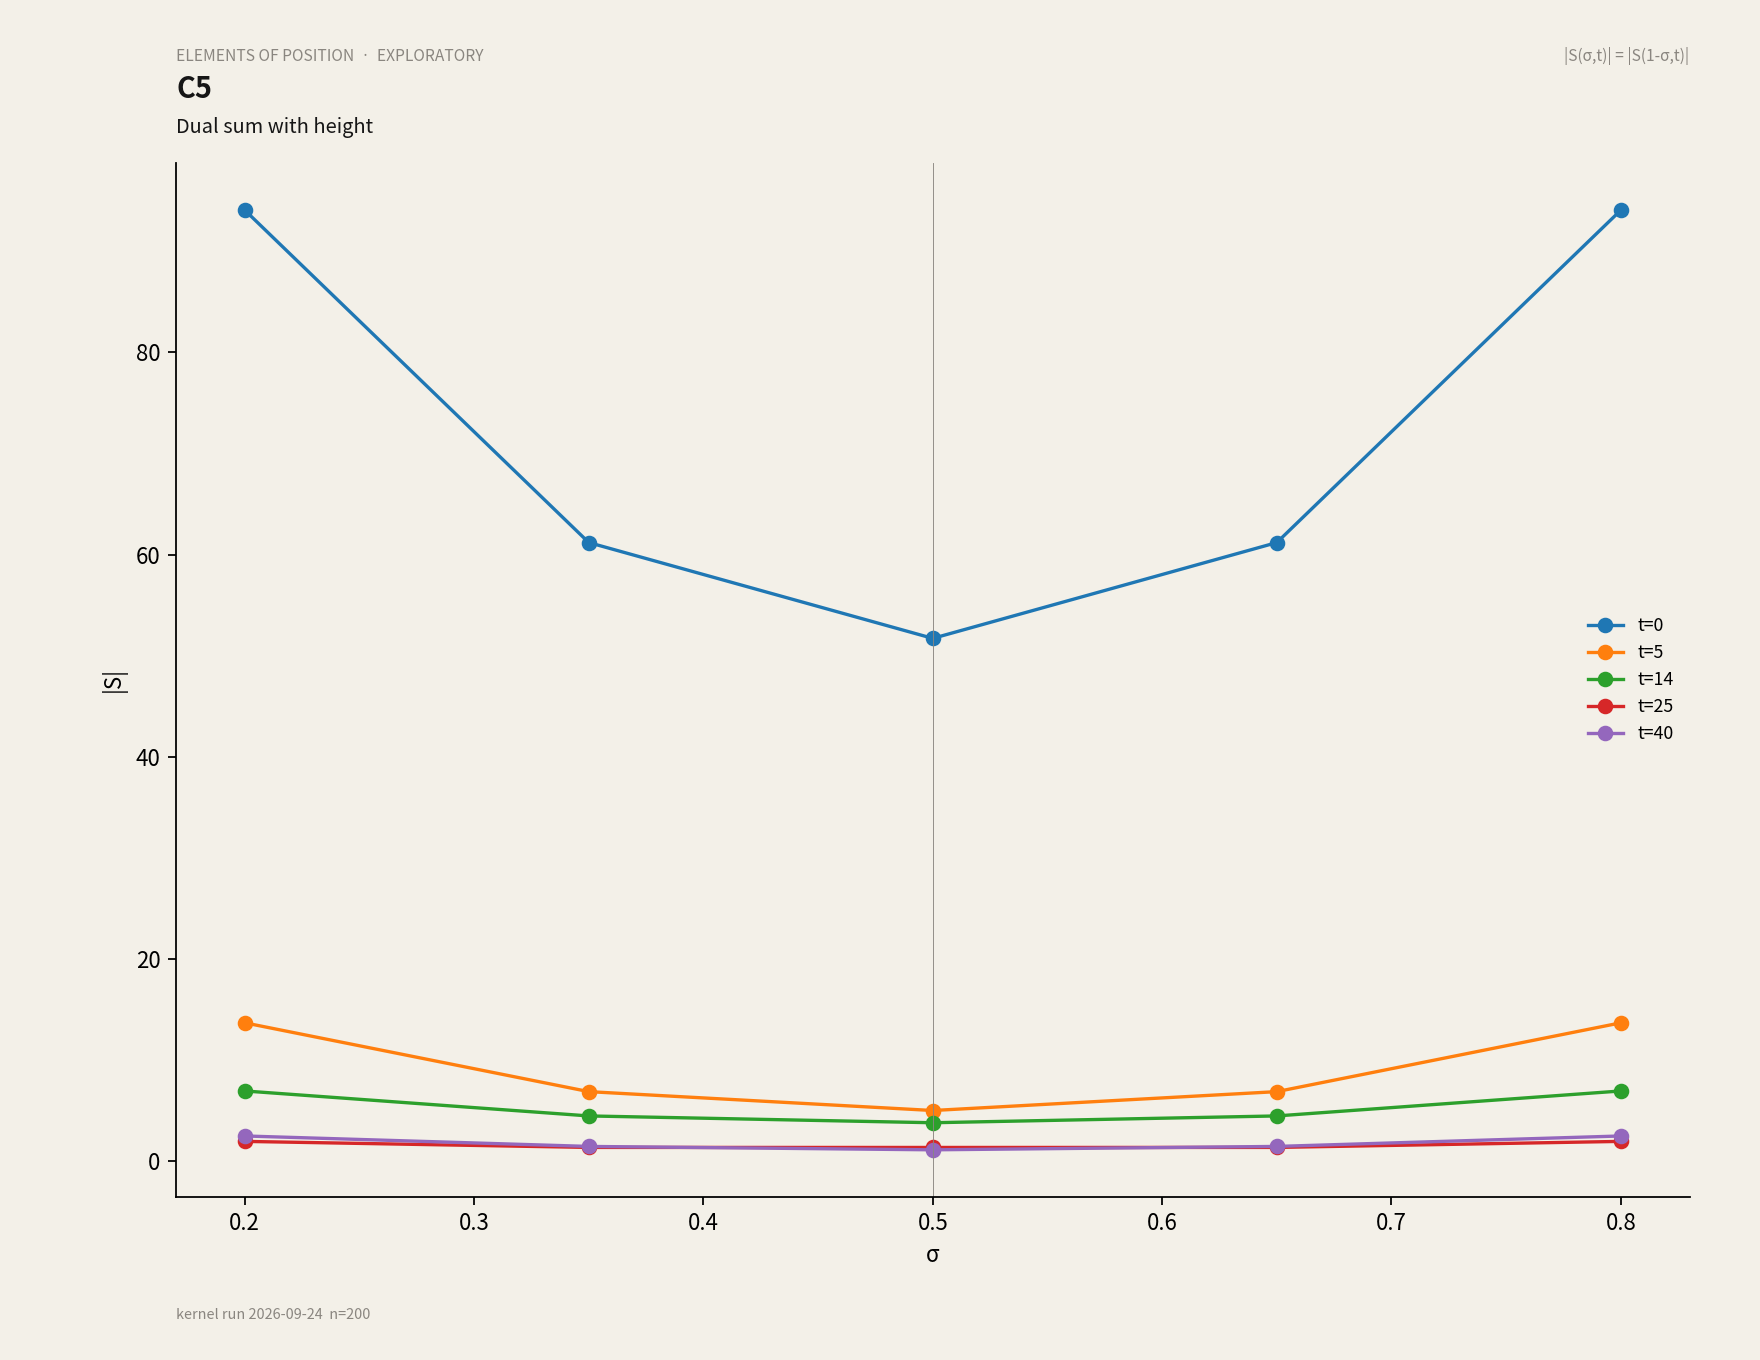
\includegraphics[width=0.92\textwidth]{C5_dual_height.png}
\caption{Sheet C5. $|S(\sigma,t)|$ on the first $t$-grid. No ordinate is claimed.}
\end{figure}

\section{A pause is one centre}

Write \(\chi(s)\) for the ratio of local-circle samples at \(1-s\) and \(s\).
For real height,
\[
\lvert\chi(\sigma+it)\rvert=1\quad\text{if and only if}\quad\sigma=\tfrac12.
\]
Off the lock, \(\lvert\chi\rvert\) is the ratio of two radii, two own-origins.
The kernel proxy \(n^{1-2\sigma}\) equals \(1\) only on the cut (\texttt{one\_centre.csv}).

\begin{figure}[htbp]
\centering
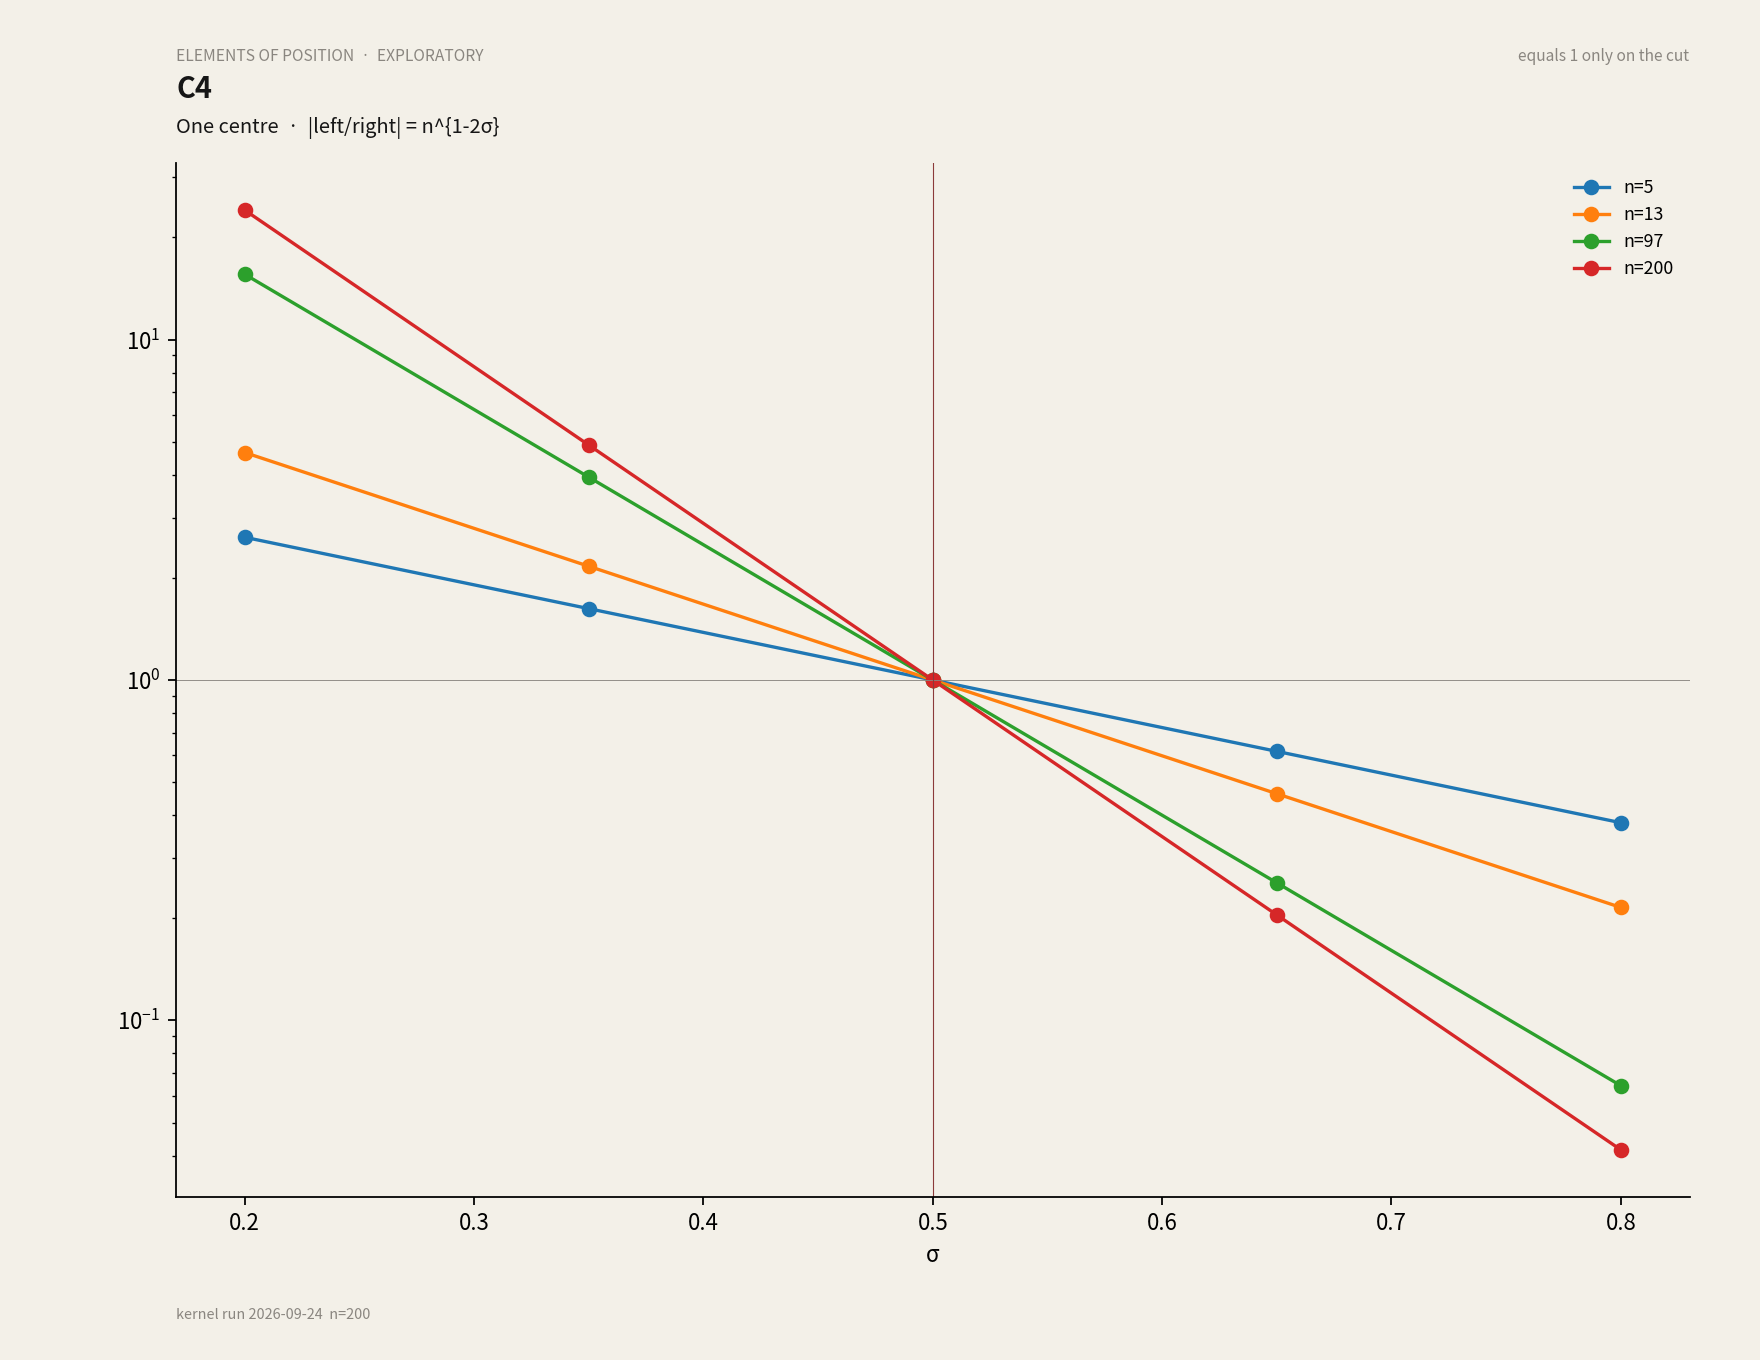
\includegraphics[width=0.92\textwidth]{C4_one_centre.png}
\caption{Sheet C4. Two-radii ratio. It is $1$ only on the cut.}
\end{figure}

A pause occupies one own-origin.
The count does not seat two centres at once.
Therefore a pause-reading has one circle, hence \(\lvert\chi\rvert=1\), hence \(\sigma=1/2\).

The off-lock dual sum, with \(\chi\) compensating unequal ends so they can still add to zero, is two centres named at once.
Vacuum may name it.
Trace cannot walk it.
A vanishing is an arrival.

\begin{theorem}[One centre]
A vanishing written as a pause-reading has \(\lvert\chi\rvert=1\), hence \(\sigma=1/2\).
Combined with the weights lemma, the two ends meet only at half.
\end{theorem}

\section{Meetings sit on the cut}

\begin{definition}[Derived unit]
The derived unit is the reading of plan, section, and elevation of the same finished stations, in the limit of those stations.
A meeting of that unit is a vanishing of a formula in the stock, from one HERE.
\end{definition}

\begin{lemma}
Every meeting of the derived unit that the construction can \emph{seat} has real part \(1/2\).
\end{lemma}

\begin{proof}
The only formula in the strip that can vanish is the dual sum.
A vanishing written as a pause-reading has one own-origin, hence \(\sigma=1/2\).
An off-lock pair \(\{\rho,1-\rho\}\) is named by the pairing \(s\leftrightarrow 1-s\).
Naming is vacuum.
To seat the pair as a meeting the construction would have to occupy two own-origins at once.
It does not.
\end{proof}

\begin{theorem}[Midline]
Every meeting of the derived unit has real part \(1/2\).
\end{theorem}

\begin{proof}
A meeting of the derived unit is a seated vanishing from one HERE.
Every meeting the construction can seat has real part \(1/2\).
An unseated name is not a meeting of the unit.
\end{proof}

\section{The identification}

The theorem above is a statement about this derived unit.
It proves nothing about any object outside the stock until a name is granted.

When the three drawings are read together through finished stations, the dated product is the Euler product on \(\operatorname{Re}s>1\); the local-circle sample is the archimedean factor; the pairing \(s\leftrightarrow 1-s\) is inversion on the index; the dual sum is the writing that can vanish in the strip.

That reading may be called by its classical name.
The name is not an ingredient of I--V.
It is granted only after the drawings exist together.

Under that identification the Midline Theorem reads as: every non-trivial zero of that limit has real part \(1/2\).

Two sentences, kept apart.
One is forced inside the stock.
One is the filing.

\section{Where \(1\) is}

Where is \(1\)?
Point to it.

It is the lock of I.
It is THERE: the elected unit, the comparison that has arrived.
We are HERE: this pause, this finished count, this own-origin.
Arrive at THERE and you are HERE --- same place, other writing.

Infinity is not a last tick of the count.
It is already the interior of \((0,1)\), and the other pole of the lock, and every finite package asked again.
No tempo reaches a different kind of mark.

II's other street was that interior asked as a process.
IV's marriage sat on the even cut.
The meetings that can be seated sit on that same line, because there is no other primary ratio for them to occupy.

The first sentence asked a location.
The location is the arrival.
The arrival is the unit.
The unit was the question.

\section{What stands}

Forced, given I--V and the stock of this paper:
the only primary self-ratio on a segment is \(1/2\);
a pause is one own-origin;
complementary interiors meet if and only if \(\sigma=1/2\);
the real dual sum meets its floor only at half (\(N=200\): \(51.7185\ldots\));
the dated product at every recorded station and height is nonzero;
the two-radii proxy equals \(1\) only on the cut;
every seated meeting of the derived unit has real part \(1/2\).

Named as identification, after the drawings exist together:
the derived unit as the classical limit of those three readings.

Not granted as an ingredient of the kernels:
a second primary ratio;
two centres at one pause;
a name treated as a seat;
a live half-walk treated as a meeting of the derived unit;
infinity as a last index;
this paper as a replacement for I--V.

Where is \(1\)?
On the cut.
Walk there and you are HERE.

\end{document}
